% =============================================================================
%  فصل پنجم — گسترش چارچوب به مسئله مجموعه احاطه‌گر کامل
%  همه اعداد این فصل از خروجی‌های ذخیره‌شده در results/tdsp بازخوانی شده‌اند.
%  مولد جدول‌ها و شکل‌ها: experiments/tdsp/ch5_report.py و ch5_example.py
% =============================================================================
\chapter{گسترش چارچوب به مسئله مجموعه احاطه‌گر کامل}
\label{ch:tdsp}

\section{مقدمه و صورت مسئله}
\label{sec:tdsp-intro}

فصل چهارم چارچوب مرجع \lr{Chen} و همکاران را بازسازی کرد؛ در آن چارچوب، مسئله
\emph{مجموعه احاطه‌گر} (\lr{DSP}) حل می‌شود: زیرمجموعه‌ای از رأس‌ها انتخاب می‌شود
که هر رأس گراف یا خود در آن مجموعه باشد یا حداقل یک همسایه در آن داشته باشد.
پرسش این فصل، نسخه سخت‌گیرانه‌تر همان مسئله است.

\begin{definition}[مجموعه احاطه‌گر کامل]
\label{def:tds}
برای گراف بدون جهت $G=(V,E)$، مجموعه $S\subseteq V$ یک \emph{مجموعه احاطه‌گر کامل}
(\lr{TDS}) است اگر هر رأس $v\in V$ حداقل یک همسایه در $S$ داشته باشد:
\begin{equation}
\forall v \in V:\quad N(v)\cap S \neq \emptyset .
\label{eq:tds-def}
\end{equation}
عدد احاطه‌گری کامل $\gamma_t(G)$ کمینه اندازه چنین مجموعه‌ای است.
\end{definition}

تفاوت با \lr{DSP} در یک واژه است: در \lr{DSP} رأس می‌تواند «خودش» نیاز را برآورده
کند، اما در \lr{TDSP} باید \emph{همسایه‌ای درون مجموعه} داشته باشد. سه پیامد
فوری این تفاوت:

\begin{enumerate}
  \item هیچ رأس منزوی نمی‌تواند در جوابی معتبر حضور داشته باشد؛ بنابراین گراف باید
        درجه کمینه حداقل یک داشته باشد و در محاسبات این فصل گراف‌های دارای رأس منزوی
        کنار گذاشته می‌شوند.
  \item هر عضو $S$ باید «پشتیبان» داشته باشد: رأسی که آن را احاطه کند. پس خروجی
        نمی‌تواند مجموعه‌ای مستقل باشد.
  \item شرط پایان فرآیند تصمیم‌گیری عوض می‌شود: در \lr{DSP} پایان یعنی «همه رأس‌ها
        پوشش داده شده‌اند»؛ در \lr{TDSP} یعنی «همه رأس‌ها همسایه‌ای در $S$ دارند»،
        و این دو نه‌فقط متفاوت، بلکه برای رأس‌های عضو مجموعه ناسازگارند.
\end{enumerate}

هر دو مسئله \lr{NP}-سخت‌اند و در ادبیات، \lr{TDSP} معادل دقیق یک مسئله
\emph{پوشش مجموعه‌ای} است: جهان، مجموعه رأس‌هاست و برای هر رأس $u$ یک مجموعه
$N(u)$ تعریف می‌شود؛ انتخاب $u$ تمام اعضای $N(u)$ را می‌پوشاند. این مشاهده،
هم خط مبنای قوی فصل (الگوریتم \lr{GRASP}) را ممکن می‌کند و هم پالایش خروجی در
بخش~\ref{sec:boosts} را.

معیارهای ارزیابی این فصل: اندازه خروجی نسبت به بهینه $\gamma_t$ و نسبت به
خط مبنای حریصانه، نسبت به بازارزیابی (\lr{GRASP})، نرخ شدنی‌بودن، تعداد تصمیم‌های
عامل و زمان استنتاج.

\section{ساخت دومرحله‌ای و کران $2|D|$}
\label{sec:construction}

اولین پرسش طبیعی این است: آیا می‌توان \lr{TDSP} را از \lr{DSP} ساخت؟ اگر $D$ یک
مجموعه احاطه‌گر معمولی باشد، آیا می‌توان از آن یک مجموعه احاطه‌گر کامل ساخت؟

برای هر $D$ یک زیرمجموعه $A\subseteq D$ با این خاصیت انتخاب می‌کنیم که هر عضو
$D$ حداقل یک همسایه در $A$ داشته باشد (مسئله‌ای در اندازه خودِ $D$)، و
$S=A\cup (V\setminus D)$ را برمی‌گردانیم.

\begin{theorem}
\label{thm:bound}
برای هر مجموعه احاطه‌گر $D$ از گرافی بدون رأس منزوی، مجموعه $S=A\cup(V\setminus D)$
یک مجموعه احاطه‌گر کامل است و
\begin{equation}
|S| \le 2|D| .
\label{eq:bound}
\end{equation}
\end{theorem}

\begin{proof}
هر $u\in V\setminus D$ چون $D$ احاطه‌کننده است، همسایه‌ای در $D$ دارد و همان همسایه
در $S$ حضور دارد (چون $A\subseteq S$). هر $u\in D$ بنا به تعریف $A$ همسایه‌ای در
$A\subseteq S$ دارد. پس شرط \eqref{eq:tds-def} برای همه رأس‌ها برقرار است. برای
اندازه: $|S|\le |A|+|V\setminus D|\le |D|+(n-|D|)$؛ کران را نمی‌توان با این
استدلال دقیق‌تر کرد، ولی در گراف‌های چگال $|V\setminus D|$ کوچک است و کران
عملاً شل می‌ماند.
\end{proof}

شکل~\ref{fig:construction} کیفیت این ساخت را به‌ازای سه منبع برای $D$ نشان می‌دهد:
حل دقیق، حریصانه، و شبکه فصل چهارم. نتیجه‌ها دو نکته را روشن می‌کنند: نخست،
کران \eqref{eq:bound} در \emph{هیچ} نمونه‌ای نقض نشد (با \lr{assert} روی همه
گراف‌ها بررسی شد)؛ دوم، کیفیت میانی بسیار بدتر از کران است، به‌ویژه روی گراف‌های
\lr{BA} که $|D|$ بزرگ است و $D$ مستقل، خروجی را تا حدود $2.7\gamma_t$ می‌برد.
به زبان دیگر، مزیت این مسیر «تضمین» است، نه «کیفیت»؛ و همین مشاهده ما را به
بازطراحی مستقیم فضای عمل سوق داد.

\begin{figure}[ht]
  \centering
  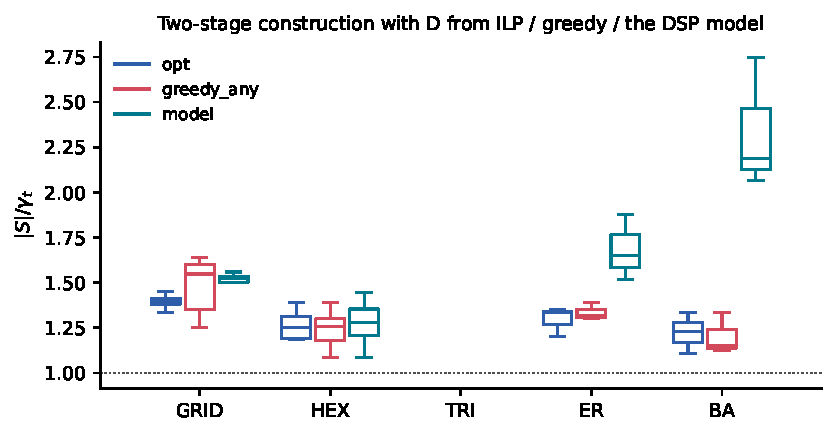
\includegraphics[width=0.85\textwidth]{figs/fig5_2_construction.pdf}
  \caption{کیفیت ساخت دومرحله‌ای ($|S|/\gamma_t$) به تفکیک خانواده گراف و منبع
  مجموعه $D$. خط‌چین، مرز بهینگی است.}
  \label{fig:construction}
\end{figure}

\section{چرا ماسک عمل مقاله برای \lr{TDSP} کار نمی‌کند؟}
\label{sec:mask}

در چارچوب مرجع، عمل مجاز فقط رأسی است که هنوز احاطه نشده باشد
($vf_v=0$)، و انتخاب $v$ خودِ $v$ و همسایه‌هایش را «احاطه‌شده» علامت می‌زند.
از این دو قاعده یک نتیجه ساختاری به‌دست می‌آید.

\begin{theorem}[ناسازگاری ماسک]
\label{thm:mask}
هر اجرای کامل سیاست مقاله (با هر قاعده انتخاب، تصادفی یا حریصانه) مجموعه‌ای
\emph{مستقل} تولید می‌کند، و بنابراین هیچ‌گاه یک مجموعه احاطه‌گر کامل نیست.
\end{theorem}

\begin{proof}
فرض کنید $u,v\in S$ و $\{u,v\}\in E$. چون $v$ با انتخاب $u$ احاطه شده است،
$vf_v=1$ می‌شود و در گام‌های بعدی $v$ از مجموعه اعمال مجاز حذف می‌شود؛ پس $v$
نمی‌تواند انتخاب شود. این با $v\in S$ در تناقض است؛ بنابراین $S$ مستقل است.
در مجموعه مستقل، هیچ عضو $S$ همسایه‌ای در $S$ ندارد، پس شرط \eqref{eq:tds-def}
برای اعضای $S$ برقرار نمی‌شود.
\end{proof}

شکل~\ref{fig:actionspace} این قضیه را تجربی تأیید می‌کند: روی \num{177} گراف از پنج
خانواده، هر سه سیاست (تصادفی، حریصانه، مدل آموزش‌دیده) خروجی مستقل دادند و
\emph{هیچ} خروجی احاطه‌گر کامل نبود. این نتیجه یک تفاوت مهم با «بدتر بودن
عملکرد» دارد: مسئله اینجا \emph{ناشدنی بودن} است، نه کیفیت پایین. پس نمی‌توان
ماسک مقاله را بدون تغییر به \lr{TDSP} منتقل کرد.

\begin{figure}[ht]
  \centering
  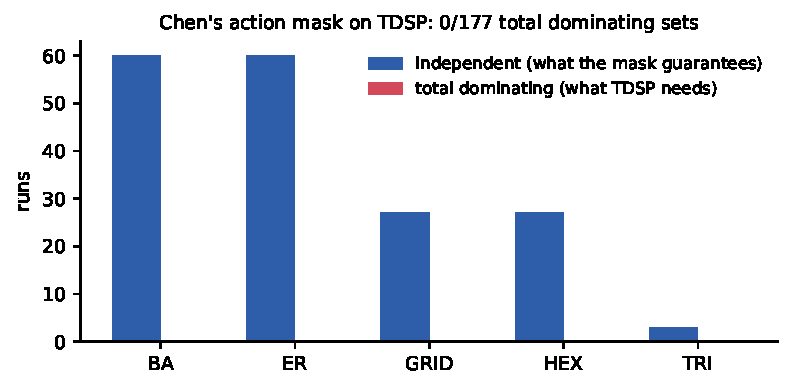
\includegraphics[width=0.8\textwidth]{figs/fig5_1_action_space.pdf}
  \caption{خروجی ماسک مقاله روی \lr{TDSP}: همه اجراها مجموعه مستقل‌اند و هیچ‌کدام
  احاطه‌کننده کامل نیست.}
  \label{fig:actionspace}
\end{figure}

کوچک‌ترین مثال نقض، مسیر $P_4$ با رأس‌های $0-1-2-3$ است. سیاست ماسک‌دار حریصانه
$S=\{1,3\}$ را می‌سازد؛ این مجموعه احاطه‌گر است و اندازه‌اش هم $2$ است، اما
رأس $3$ هیچ همسایه‌ای در $S$ ندارد، چون تنها همسایه‌اش ($2$) عضوی از مجموعه نیست.
در همین گراف، جواب بهینه مجموعاً برابر $2$ است ولی با ترکیب دیگری
($S^\ast=\{1,2\}$). شکل~\ref{fig:p4} این مغایرت را نشان می‌دهد: تفاوت در اندازه
نیست، در \emph{شدنی‌بودن} است.

\begin{figure}[ht]
  \centering
  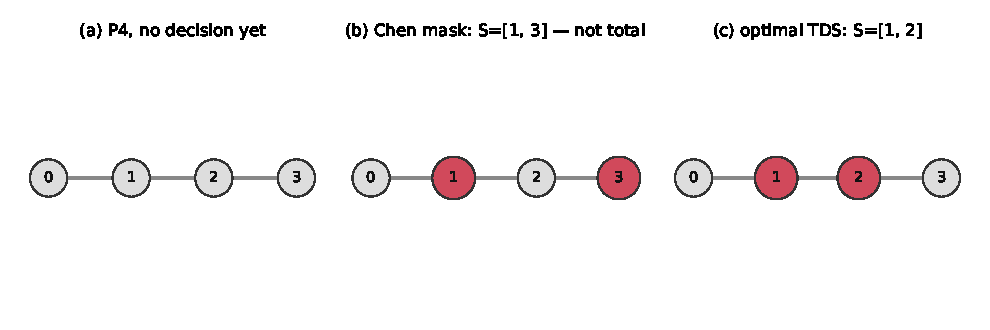
\includegraphics[width=0.92\textwidth]{figs/fig5_11_p4.pdf}
  \caption{مثال نقض روی $P_4$: (الف) گراف؛ (ب) خروجی ماسک مقاله
  ($S=\{1,3\}$) که احاطه‌گر کامل نیست؛ (ج) جواب بهینه $\{1,2\}$ با همان اندازه.}
  \label{fig:p4}
\end{figure}

\section{محیط بازطراحی‌شده: فضای عمل \lr{TDSP}}
\label{sec:env}

بر اساس بخش~\ref{sec:mask}، سه قاعده چارچوب مرجع بازنویسی می‌شود:

\begin{enumerate}
  \item \textbf{ماسک:} هر رأسی که هنوز در $S$ نیست مجاز است (نه فقط رأس‌های
        احاطه‌نشده). بنابراین اعضای $S$ می‌توانند همسایه یکدیگر باشند.
  \item \textbf{گذار:} انتخاب $v$ فقط $N(v)$ را «راضی» می‌کند و خودِ $v$ راضی
        نمی‌شود؛ پس $vf_v$ تا زمانی که همسایه‌ای انتخاب نشود صفر می‌ماند. این
        قاعده، قید احاطه‌گری کامل را به‌صورت بومی در مکانیک مسئله می‌نشاند.
  \item \textbf{پایان:} فرآیند وقتی پایان می‌یابد که همه رأس‌ها
        $vf=1$ باشند، یعنی هر رأس همسایه‌ای در $S$ داشته باشد.
\end{enumerate}

از آنجا که در مسئله جدید «عضو بودن» و «احاطه‌شده بودن» دو چیز متفاوت‌اند،
حالت محیط باید دو کانال داشته باشد:
\begin{equation}
s = \big[\,vf \;\|\; ins\,\big] \in \{0,1\}^{n\times 2},
\qquad
vf_u = \mathbb{I}\big[N(u)\cap S \neq \emptyset\big],
\qquad
ins_u = \mathbb{I}\big[u \in S\big].
\label{eq:state}
\end{equation}
اگر تنها $vf$ به شبکه داده شود، دو وضعیت متمایز (رأسی که انتخاب شده ولی هنوز
راضی نشده، و رأسی که نه انتخاب شده و نه راضی است) یکسان دیده می‌شوند و سیاست
نمی‌تواند میان آن‌ها تفکیک کند. شکل~\ref{fig:trace} (الف) و (ب) همین دو کانال را
روی یک مثال نشان می‌دهد.

نکته مهم برای بازتولید: رابط محیط ($reset/candidates/step$) عوض نشده است؛ فقط
\emph{قواعد} و \emph{ابعاد حالت} تغییر کرده‌اند. بنابراین حلقه یادگیری، شبکه
پیام‌رسان و مکانیزم \lr{DDQN} فصل چهارم بدون بازنویسی روی محیط جدید کار می‌کنند؛
تنها شرط آن است که نامزدها از خود محیط خوانده شوند (نه از $vf=0$) و شبکه
$in-ch=2$ بگیرد. سه آزمون مستقل این تطبیق را تأیید کرد: \num{118} بررسی مکانیک،
هم‌ارزی سیاست حریصانه محیط با \lr{greedy} بومی در \num{59} از \num{59} نمونه،
و بازتولید خط‌به‌خط نتایج \lr{DSP} فصل چهارم با نسخه پیشین کد (آزمون عدم رگرسیون).

\section{تابع پاداش: از «سود» به «هزینه هر تصمیم»}
\label{sec:reward}

پاداش چارچوب مرجع بر پایه تعداد رأس‌های تازه‌احاطه‌شده تعریف می‌شود. روی
\lr{TDSP} این تعریف یک اشکال ساختاری پیدا می‌کند.

\begin{theorem}
\label{thm:gain}
اگر پاداش هر گام برابر تعداد رأس‌هایی باشد که با انتخاب آن گام تازه راضی
می‌شوند (پاداش سود، یا نسخه $\pm 1$ مقاله)، بازدهی هر اپیزود مستقل از سیاست و
از اندازه مجموعه نهایی است.
\end{theorem}

\begin{proof}
شرط پایان محیط این است که همه رأس‌ها $vf=1$ شوند. هر رأس در پایان اپیزود
دقیقاً یک‌بار «تازه راضی‌شده» شمرده می‌شود؛ بنابراین مجموع سود در طول اپیزود
همیشه برابر $n$ است و بازده $n$ (یا ترکیب خطی ثابت از $n$) می‌شود، مستقل از
$|S|$.
\end{proof}

نتیجه: عاملی که این پاداش را بیشینه می‌کند هیچ انگیزه‌ای برای کوچک کردن $|S|$
ندارد؛ همه سیاست‌ها بازده یکسان می‌گیرند و سیگنال بهینه‌سازی از بین می‌رود.

\begin{definition}[پاداش هزینه]
\label{def:size-reward}
در هر تصمیم عامل پاداش $r=-1$ می‌گیرد. بنابراین بازده اپیزود برابر
$-|\text{تصمیم‌های عامل}|$ است، و اگر مجموعه اجباری $F$ (بخش~\ref{sec:forcing})
از پیش در $S$ باشد، بازده کل برابر $-|S|$ می‌شود.
\end{definition}

جدول~\ref{tab:reward} این تفاوت را روی مثال بخش~\ref{sec:example} عددگذاری می‌کند.
در سطح کل آزمایش‌ها، این تغییر ساده اثر چشمگیری داشت: میانگین
$|S|/\text{greedy}$ روی گراف‌های تصادفی بزرگ از $4.34$ به $1.04$ رسید و
مدل از «شش برابر بدتر از حریصانه» به «هم‌سطح آن» تغییر کرد؛ روی لتیس‌های
شش‌گوش، پاداش \lr{paper} کمی بهتر از پاداش هزینه بود ($0.812$ در برابر
$0.877$).

\begin{table}[ht]
  \centering
  \caption{دو تابع پاداش روی مثال گراف درختی $n=12$ (بخش~\ref{sec:example})}
  \label{tab:reward}
  \begin{tabular}{lccc}
    \toprule
    پاداش & بازده اپیزود & ارتباط با هدف & سیگنال بهینه‌سازی \\
    \midrule
    سود (نسخه مقاله) & $+12$ & مستقل از $|S|$ & ندارد \\
    هزینه ($r=-1$) & $-6$ & دقیقاً $-|S|$ & دارد \\
    \bottomrule
  \end{tabular}
\end{table}

\section{معماری شبکه: یک باگ مقیاس‌پذیری و رفع آن}
\label{sec:arch}

خوانش گراف در چارچوب مرجع، جمع نمایش رأس‌ها است: $s=\sum_{u} h_u$. این تعریف
برای $n$ ثابت بی‌ضرر است، ولی وقتی مدل فقط روی $n=20$ آموزش می‌بیند و روی
اندازه‌های دیگر آزمون می‌شود، فاجعه‌بار می‌شود: اندازه خروجی خوانش با $n$ رشد
می‌کند و مقادیر $Q$ منفجر می‌شوند. اندازه‌گیری ما: در $n=20$ مقدار $Q\approx0.8$
بود و در $n=300$ به $85183$ می‌رسید. این باگ در مسئله \lr{DSP} نیز وجود داشت
($Q\approx76379$ در $n=500$)، ولی چون مقاله برای هر اندازه یک مدل جدا آموزش
می‌دهد، در گزارش اصلی آشکار نشده است.

رفع باگ دو تغییر کوچک است: تابع تجمیع پیام‌ها از جمع به \emph{میانگین}
($\text{agg}=\text{mean}$) و خوانش گراف از $\sum h_u$ به $\frac1n\sum h_u$
($\text{mean-readout}$). پس از این تغییر، $Q$ برای همه اندازه‌ها تقریباً ثابت
می‌ماند ($\approx0.09$) و تعمیم به اندازه‌های آموزش‌ندیده ممکن می‌شود.
شکل~\ref{fig:arch} اثر این اصلاح را نشان می‌دهد: روی گراف‌های تصادفی با
$n\ge 80$ کیفیت مدل با پاداش هزینه از $4.34$ به $1.04$ بهبود می‌یابد و روی
لتیس‌ها مدل بهتر از حریصانه می‌شود ($0.81$–$0.88$).

\begin{figure}[ht]
  \centering
  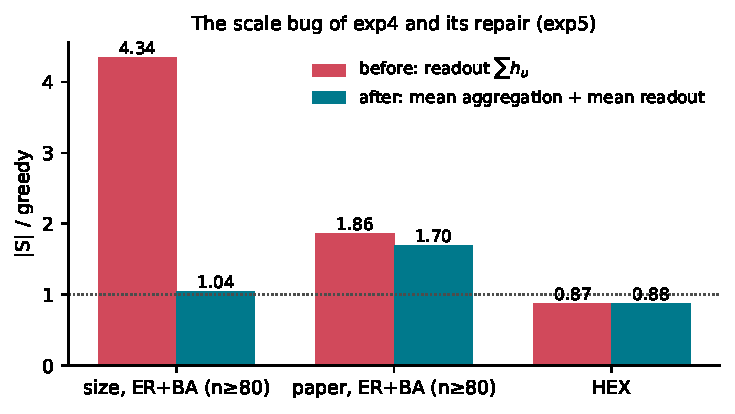
\includegraphics[width=0.72\textwidth]{figs/fig5_3_architecture.pdf}
  \caption{اثر رفع باگ مقیاس‌پذیری خوانش گراف بر کیفیت مدل.}
  \label{fig:arch}
\end{figure}

\section{دانش گراف: قواعد کاهش و اجبار برگ‌ها}
\label{sec:forcing}

نوآوری دوم پروپوزال، استفاده از مفاهیم نظریه گراف برای کاهش فضای جست‌وجو است.
سه قاعده کلاسیک بررسی شد:

\begin{enumerate}
  \item \textbf{رأس منزوی:} تنها برای تشخیص ناشدنی‌بودن مفید است.
  \item \textbf{مؤلفه‌های همبند:} تجزیه دقیق است و مسئله را به مؤلفه‌ها می‌شکند.
  \item \textbf{برگ و پشتیبان:} در \lr{DSP} معتبر است، اما در \lr{TDSP}
        \emph{نامعتبر} است.
\end{enumerate}

\begin{theorem}[نامعتبری قاعده برگ]
\label{thm:leaf-invalid}
در \lr{TDSP} نمی‌توان رأس پشتیبان یک برگ و همسایگانش را از گراف حذف کرد و
مسئله را روی گراف باقی‌مانده حل کرد.
\end{theorem}

\begin{proof}
مثال نقض: مسیر $P_3$ با رأس‌های $0-1-2$. برگ $0$ رأس $1$ را اجباری می‌کند. با
حذف $\{1\}\cup N(1)=\{0,1,2\}$ گراف خالی می‌ماند و جواب پیشنهادی $\{1\}$ است؛
اما $1$ هیچ همسایه‌ای در مجموعه ندارد و احاطه‌گری کامل برقرار نیست. جواب بهینه
$\{0,1\}$ با اندازه $2$ است. علت ساختاری: در احاطه‌گری کامل، خودِ رأس پشتیبان هم
باید پشتیبان داشته باشد، پس زیرمسئله، گراف القایی ساده نیست.
\end{proof}

پس قاعده برگ به شکل «حذف» بی‌اعتبار است. اما شکل \emph{مثبت} همان ایده معتبر است:
هر پشتیبانِ برگ در \emph{هر} جواب معتبر حاضر است، چون تنها همسایه برگ خودش است
و برگ باید توسط آن احاطه شود.

\begin{definition}[مجموعه اجباری]
\label{def:forced}
$F$ را مجموعه پشتیبان‌های برگ‌ها بگیرید. چون هر برگ درجه یک دارد، پشتیبانش در
هر مجموعه احاطه‌گر کامل حاضر است.
\end{definition}

ایده اجرایی: به‌جای حذف رأس‌ها، $F$ را در \emph{ابتدای اپیزود} در $S$ می‌نشانیم.
مکانیک $vf$ خودبه‌خود قید باقی‌مانده را حمل می‌کند: هر عضو $F$ چون خودش هم باید
پشتیبان داشته باشد، همچنان «راضی‌نشده» می‌ماند و عامل باید برایش همسایه انتخاب
کند. پاداش هزینه فقط به تصمیم‌های عامل تعلق می‌گیرد و چون $|F|$ در هر جواب
ثابت است، آفستی ثابت است و بهینه‌سازی را تغییر نمی‌دهد.

چرا این مسیر روی خانواده‌های متراکم بی‌اثر است؟ چون آن گراف‌ها برگ ندارند
($F=\emptyset$) و لتیس‌ها هم تک‌مؤلفه‌ای و بدون رأس منزوی‌اند؛ بنابراین قاعده‌های
یک و دو هم فعال نمی‌شوند. یعنی قواعد کاهش کلاسیک در این دامنه سودی ندارند — یک
نتیجه منفی که صادقانه گزارش می‌شود. اما روی خانواده‌های \emph{اسپارس} (درخت
تصادفی و \lr{BA} با $m=1$) وضعیت فرق می‌کند: پوشش $F$ تا حدود $30\%$ رأس‌ها را
می‌گیرد و صرفه‌جویی بزرگی در تعداد تصمیم ایجاد می‌کند.

جدول~\ref{tab:forcing} و شکل~\ref{fig:rlsteps} این صرفه‌جویی را نشان می‌دهند:
روی درخت‌ها، تعداد تصمیم‌های عامل برای $n=100$ از $46.6$ به $16.2$ و برای
$n=200$ از $94.3$ به $34.1$ می‌رسد (کاهش حدود $64\%$)، بدون آنکه کیفیت نهایی
تغییر کند.

\begin{table}[ht]
  \centering
  \caption{اثر اجبار برگ‌ها روی کیفیت و تعداد تصمیم (درخت تصادفی یکنواخت)}
  \label{tab:forcing}
  \begin{tabular}{lccccc}
    \toprule
    پیکربندی & $|S|/\gamma_t$ ($n=100$) & تصمیم‌ها ($n=100$) & $|S|/\gamma_t$ ($n=200$) & تصمیم‌ها ($n=200$) \\
    \midrule
    سیاست آزاد & $1.000$ & $46.6$ & $1.000$ & $94.3$ \\
    سیاست با $F$ & $1.000$ & $16.2$ & $1.000$ & $34.1$ \\
    \bottomrule
  \end{tabular}
\end{table}

\begin{figure}[ht]
  \centering
  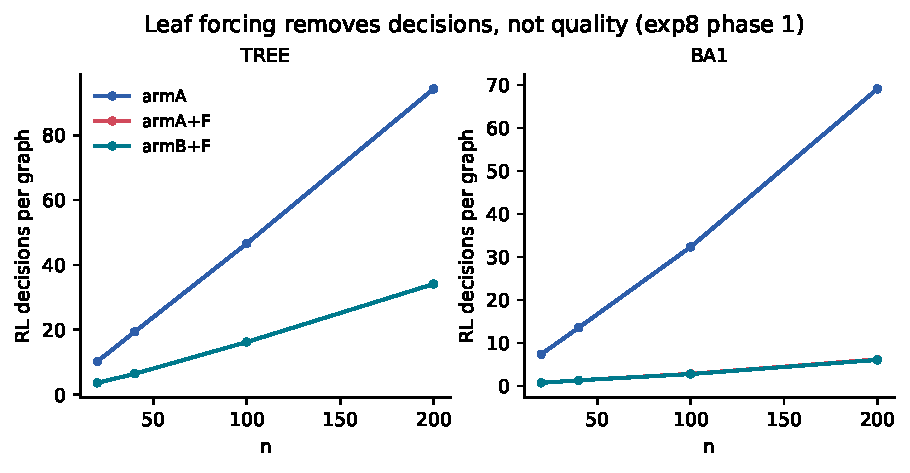
\includegraphics[width=0.85\textwidth]{figs/fig5_8_rl_steps.pdf}
  \caption{تعداد تصمیم‌های عامل به‌ازای هر گراف، با و بدون اجبار برگ‌ها.}
  \label{fig:rlsteps}
\end{figure}

اثر اجبار روی \emph{همگرایی} نیز اندازه‌گیری شد. در آزمایش زوجی با سه seed،
هر دو بازو به کیفیت نهایی یکسان رسیدند
($9.67\pm0.15$) اما بازوی دارای اجبار پس از
$43{,}333\pm10{,}408$ اپیزود به این سطح رسید و بازوی بدون اجبار پس از
$160{,}000\pm18{,}028$ اپیزود؛ یعنی \emph{حدود سه و نیم برابر} سریع‌تر. این
مقایسه زوجی است، چون با seed یکسان هر دو بازو دنباله یکسانی از گراف‌های آموزش،
مقداردهی اولیه شبکه و برنامه $\varepsilon$ می‌گیرند و تنها عامل تفاوت، خودِ اجبار
است. نکته صادقانه: مدل آموزش‌دیده با اجبار باید در زمان \emph{آزمون} هم با $F$
اجرا شود؛ اگر بدون $F$ اجرا شود، روی گراف‌های اسپارس از حریصانه بدتر عمل می‌کند.

\section{الگوریتم یادگیری: از \lr{DDQN} به سر دوگانه}
\label{sec:d3qn}

پس از تثبیت محیط، پاداش و گراف، پرسش بعدی این بود که آیا «الگوریتم یادگیری
بهتر» چیزی اضافه می‌کند؟ کوچک‌ترین تغییر ممکن، سر دوگانه
(\lr{Dueling}) است که تابع ارزش را به دو بخش تجزیه می‌کند:
\begin{equation}
Q(s,v) = V(s) + A(s,v) - \frac{1}{|\mathcal{A}(s)|}\sum_{v'\in\mathcal{A}(s)} A(s,v'),
\label{eq:dueling}
\end{equation}
که $V$ ارزش حالت و $A$ مزیت عمل است. محیط، پاداش، \lr{MPNN}، قاعده به‌روزرسانی
\lr{DDQN} و پروتکل آموزش دست‌نخورده می‌مانند و فقط سر شبکه عوض می‌شود
(فلگ \lr{--dueling}، پیش‌فرض خاموش تا نتایج پیشین بی‌تغییر بمانند).

نتیجه غربالگری: کیفیت نهایی در هر چهار مقایسه زوجی عملاً یکسان است
($9.50/9.80/9.70/9.50$ در برابر $9.50/9.80/9.70/9.50$)، اما رسیدن به سطح فلات
سریع‌تر می‌شود: میانگین سه seed در بازوی آزاد از $150{,}000$ به $90{,}000$
اپیزود و در بازوی دارای اجبار از $45{,}000$ به $25{,}000$ اپیزود (حدود
$1.7$ برابر). شکل~\ref{fig:convergence} (چپ) این تفاوت را نشان می‌دهد.

\begin{figure}[ht]
  \centering
  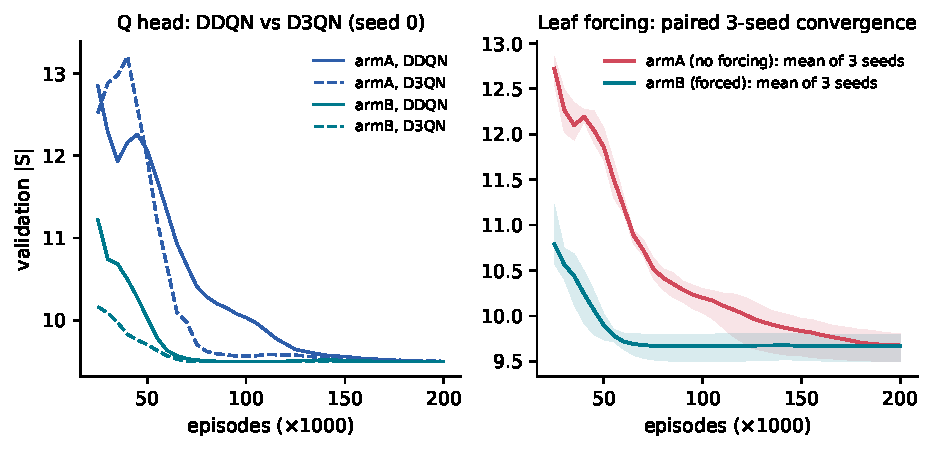
\includegraphics[width=0.95\textwidth]{figs/fig5_7_convergence.pdf}
  \caption{چپ: همگرایی \lr{DDQN} و \lr{D3QN} با seed یکسان. راست: اثر اجبار برگ
  روی میانگین سه seed با نوار کمینه–بیشینه.}
  \label{fig:convergence}
\end{figure}

حکم ما صریح است: \lr{D3QN} «بهتر نیست، ارزان‌تر است». ارزش آن صرفه‌جویی در
بودجه آموزش است، نه بهبود کیفیت پاسخ. همچنین باید توجه داشت که معیار
«اپیزود رسیدن به سطح فلات» یک معیار آستانه‌ای است؛ در یکی از seedها که مقدار
نهایی دقیقاً روی آستانه می‌نشیند، این معیار بی‌معنا می‌شود و عدد سرعت را نباید
به‌عنوان سرعت دیواری نقل کرد.

\section{دو تقویت صفر-آموزش}
\label{sec:boosts}

تا اینجا هر بهبود هزینه آموزش داشت. پرسش آخر این بود: از checkpointهای موجود،
بدون هیچ آموزش تازه، چقدر می‌توان گرفت؟ دو تقویت بررسی شد.

\subsection{پالایش خروجی (\lr{remove-redundant})}

چون \lr{TDSP} دقیقاً یک مسئله پوشش مجموعه‌ای است، پالایش کلاسیک روی \emph{هر}
جواب معتبر قابل اعمال است: اگر رأسی در $S$ باشد که همه همسایه‌هایش توسط
اعضای دیگر $S$ پوشش داده می‌شوند، حذف آن جواب را از احاطه‌گری کامل خارج
نمی‌کند.

\begin{lemma}
\label{lem:rr}
اگر $S$ احاطه‌گر کامل باشد و $v\in S$ حذف شود، مجموعه حاصل احاطه‌گر کامل
است به شرط آنکه هر $u\in N(v)$ عضوی از $S\setminus\{v\}$ داشته باشد. بنابراین
اندازه هرگز افزایش نمی‌یابد و خروجی همیشه شدنی می‌ماند.
\end{lemma}

\begin{proof}
برای هر $u\in N(v)$، همسایه‌ای در $S\setminus\{v\}$ موجود است (فرض لم). برای
سایر رأس‌ها، شاهدان پیشین دست‌نخورده‌اند چون تنها $v$ حذف شده و $v$ شاهد هیچ
رأسی جز همسایه‌هایش نبود.
\end{proof}

در پیاده‌سازی، این شرط نه فرض، بلکه \emph{خودِ آزمون} است: پس از هر حذف بررسی
می‌شود که مجموعه همچنان احاطه‌گر کامل است، و همچنین \lr{assert} می‌شود که اندازه
زیاد نشود. اثر عملی چشمگیر بود (شکل~\ref{fig:refinement}): روی گراف‌های متراکم،
\lr{armA} از $1.205$ به $1.059$ (حدود $12\%$ کوچک‌تر؛ در $55\%$ نمونه‌ها حداقل یک
رأس حذف شد) و \lr{paper-v2} از $1.310$ به $1.183$ بهبود یافت. روی گراف‌های اسپارس
اثر تقریباً صفر است، چون مجموعه‌های مدل از پیش کمینه‌اند.

\begin{figure}[ht]
  \centering
  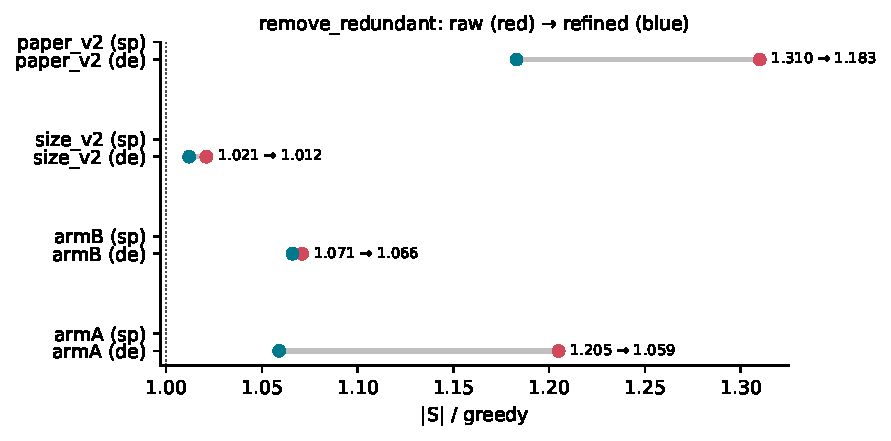
\includegraphics[width=0.62\textwidth]{figs/fig5_6_refinement.pdf}
  \caption{اثر \lr{remove-redundant} روی خروجی چهار \lr{checkpoint}.}
  \label{fig:refinement}
\end{figure}

همین پالایش یک ایراد روش‌شناختی در مقایسه‌های پیشین را آشکار کرد: در آزمایش
بازارزیابی، \lr{GRASP} \emph{درون خود} این پالایش را دارد، در حالی که مدل با
خروجی خام سنجیده می‌شد. پس از متقارن کردن این شرط، فاصله مدل و \lr{GRASP} به‌شدت
کم شد و ادعای «مدل به \lr{GRASP} می‌بازد» به «هم‌سطح» تغییر کرد.

\subsection{ماسک \lr{top-k} بر پایه سود}

در هر گام، به‌جای آنکه سیاست در میان همه رأس‌های مجاز انتخاب کند، فقط $k$ رأسِ
با بیشترین سود (تعداد همسایه‌های راضی‌نشده) قانونی اعلام می‌شوند و شبکه میان
آن‌ها انتخاب می‌کند. دو سر این طیف از پیش معلوم است: $k=1$ دقیقاً سیاست حریصانه
بومی است و $k=n$ همان سیاست آزاد. این تقویت، تعمیم عملی همان ایده «اولویت‌گذاری
نامزدها» است که در طرح اولیه دنبال می‌کردیم.

شکل~\ref{fig:topk} نتیجه جاروب را نشان می‌دهد: $k=3$ بهترین است
($1.205\rightarrow1.009$ برای \lr{armA}) و افزایش $k$ به $5$ و $10$ بدتر می‌شود.
تفسیر: سود از «حذف گزینه‌های کم‌سود» می‌آید، نه از آزادی بیشتر؛ یعنی سیاست در
گام‌هایی که یک رأس کم‌سود را ترجیح می‌دهد اشتباه می‌کند. ترکیب $k=3$ با پالایش
خروجی، مدل را به سطح \lr{GRASP} می‌رساند.

\begin{figure}[ht]
  \centering
  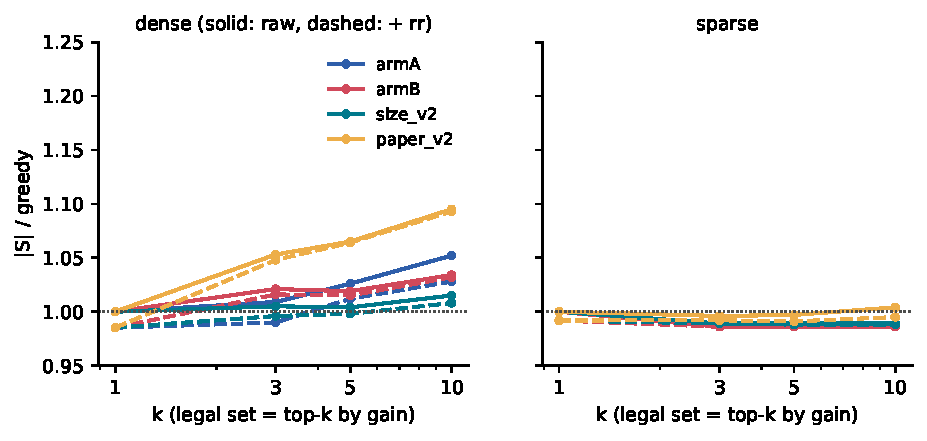
\includegraphics[width=0.95\textwidth]{figs/fig5_5_topk_sweep.pdf}
  \caption{جاروب ماسک \lr{top-k}: نسبت اندازه به حریصانه بر حسب $k$.}
  \label{fig:topk}
\end{figure}

برای آنکه ادعای «هوشمندی سیاست» با «کمک ماسک حریصانه» اشتباه نشود، دو کنترل
افزوده شد: (الف) \lr{greedy+rr}، یعنی همان پالایش روی سیاست بی‌هوش؛ (ب)
\lr{random@k+rr}، یعنی سکه‌انداختن در همان مجموعه $k$ رأسی. نتیجه
روی گراف‌های متراکم: \lr{armA@3+rr} برابر $0.990$، \lr{random@3+rr} برابر
$1.099$ و \lr{greedy+rr} برابر $0.995$؛ یعنی شبکه در همان مجموعه قانونی
$11$ واحد بهتر از سکه‌انداختن عمل می‌کند، ولی نسبت به حریصانه پالایش‌شده تقریباً
هم‌سطح است.

\section{ارزیابی جامع}
\label{sec:eval}

ارزیابی این فصل روی \num{168} نمونه گراف انجام شد: \num{88} گراف متراکم
(شبکه مستطیلی، شش‌گوش، مثلثی و \lr{ER/BA} تا $n=300$) و \num{80} گراف اسپارس
(درخت تصادفی و \lr{BA} با $m=1$ تا $n=200$)، با چهار \lr{checkpoint} و
\num{6888} مجموعه تولیدشده. همه مجموعه‌های تولیدشده یک‌بار دیگر به‌عنوان
احاطه‌گر کامل بررسی شدند: \emph{هیچ} خروجی ناشدنی وجود نداشت، هیچ‌گاه
\lr{remove-redundant} اندازه را افزایش نداد و ماسک با $k=1$ در \num{168} از
\num{168} نمونه دقیقاً همان جواب حریصانه بومی را داد (شاهد درست‌بودن پیاده‌سازی).

شکل~\ref{fig:quality} کیفیت را نسبت به حریصانه به تفکیک خانواده نشان می‌دهد و
جدول~\ref{tab:paired} نتیجه آزمون‌های زوجی را خلاصه می‌کند. آزمون‌ها روی گراف‌های
\emph{جفت‌شده} (یک شناسه برای هر گراف) انجام شده‌اند: بازه اطمینان بوت‌استرپ با
\num{10000} بازنمونه‌گیری و آزمون ویلکاکسون علامت‌دار.

\begin{table}[ht]
  \centering
  \caption{مقایسه‌های زوجی روی گراف‌های متراکم و اسپارس (معیار $|S|/|greedy|$)}
  \label{tab:paired}
  \begin{tabular}{lcccc}
    \toprule
    مقایسه & تفاوت میانگین & بازه اطمینان ۹۵٪ & $p$ & حکم \\
    \midrule
    \lr{armA@3+rr} در برابر \lr{greedy+rr} & $-0.0049$ & $[-0.019,\,+0.010]$ & $0.485$ & تساوی \\
    \lr{armA@3+rr} در برابر \lr{GRASP} & $+0.0026$ & $[-0.017,\,+0.023]$ & $0.851$ & تساوی \\
    \lr{armA@3+rr} در برابر \lr{random@3+rr} & $-0.109$ & $[-0.150,\,-0.071]$ & $1.5\times10^{-7}$ & شبکه مؤثر است \\
    \lr{armA} در برابر \lr{armA@3} & $+0.196$ & $[+0.155,\,+0.239]$ & $2\times10^{-11}$ & ماسک مؤثر است \\
    \lr{armA} در برابر \lr{armA+rr} & $+0.145$ & $[+0.110,\,+0.183]$ & $2\times10^{-9}$ & پالایش مؤثر است \\
    \lr{armB@3+rr} در برابر \lr{greedy+rr} & $+0.022$ & $[+0.004,\,+0.041]$ & $0.035$ & اندکی بدتر \\
    \lr{armA+F} در برابر \lr{GRASP} (اسپارس) & $+0.0001$ & $[0,\,+0.0004]$ & $0.317$ & تساوی \\
    \bottomrule
  \end{tabular}
\end{table}

\begin{figure}[ht]
  \centering
  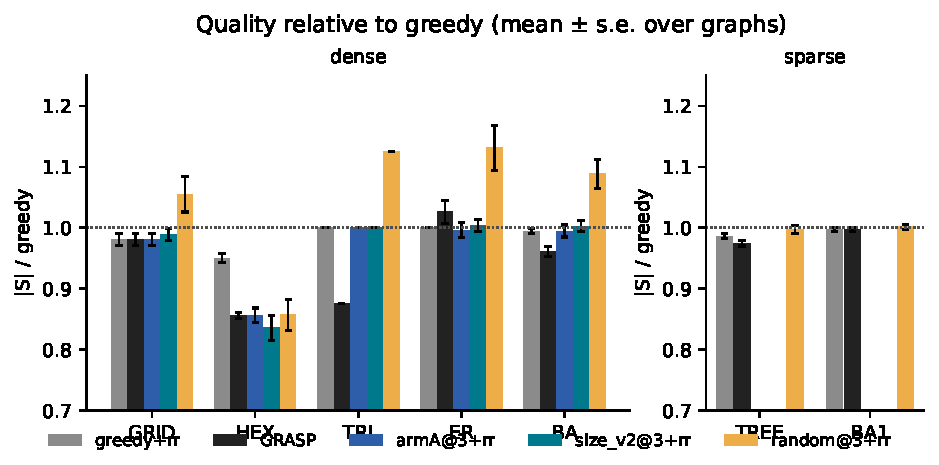
\includegraphics[width=0.98\textwidth]{figs/fig5_4_quality_by_family.pdf}
  \caption{کیفیت نسبت به حریصانه به تفکیک خانواده (میانگین $\pm$ خطای معیار).}
  \label{fig:quality}
\end{figure}

جمع‌بندی کمّی:

\begin{itemize}
  \item روی گراف‌های تصادفی متراکم، پیکربندی پیشنهادی
        (\lr{armA@3+rr}) با بازارزیابی \lr{GRASP} \emph{آماری} هم‌سطح است و
        از حریصانه پالایش‌شده هم بهتر نیست؛ برتری واقعیRL در این خانواده وجود
        ندارد و صادقانه گزارش می‌شود.
  \item روی گراف‌های اسپارس، مدل به بهینه می‌رسد
        ($|S|/\gamma_t=1.000$ برای هر دو بازوی آموزش‌دیده) و از
        \lr{greedy+rr} به‌طور آماری بهتر است ($p=4\times10^{-4}$)، هرچند
        اختلاف اندازه ناچیز است.
  \item روی لاتیس شش‌گوش، مدل \emph{واقعاً} برنده است: بهترین نتیجه فصل
        \lr{size-v2@3+rr} با نسبت $0.786$ در برابر \lr{GRASP} با $0.847$ و
        حریصانه پالایش‌شده با $0.959$ (شکل~\ref{fig:hex}).
  \item هزینه: مدل با تقویت‌ها روی گراف‌های متراکم حدود $0.015$ ثانیه و روی
        اسپارس $0.005$–$0.007$ ثانیه زمان می‌برد، در برابر $0.068$ ثانیه
        (\lr{GRASP} روی متراکم) و $0.163$ ثانیه (روی اسپارس)؛ یعنی حدود
        $4$ تا $25$ برابر سریع‌تر با کیفیت هم‌سطح (شکل~\ref{fig:timequality}).
\end{itemize}

\begin{figure}[ht]
  \centering
  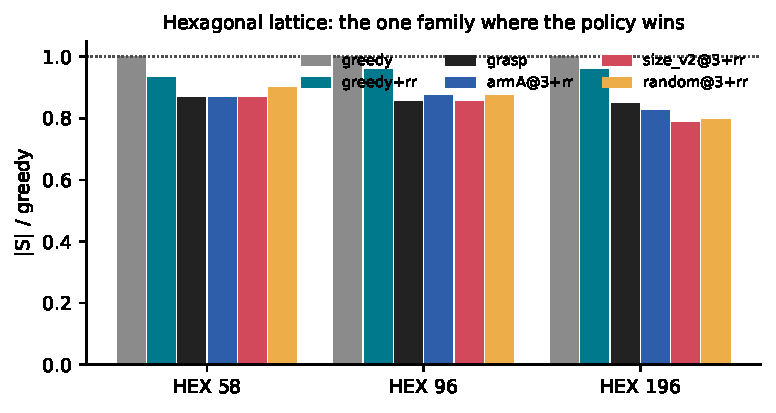
\includegraphics[width=0.72\textwidth]{figs/fig5_10_hex.pdf}
  \caption{خانواده شش‌گوش: تنها خانواده‌ای که سیاست به‌طور معنادار از
  بازارزیابی بهتر است.}
  \label{fig:hex}
\end{figure}

\begin{figure}[ht]
  \centering
  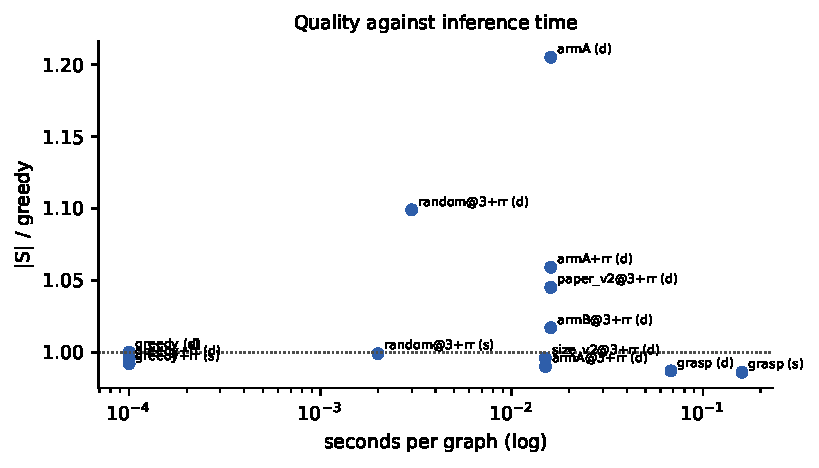
\includegraphics[width=0.72\textwidth]{figs/fig5_9_time_quality.pdf}
  \caption{کیفیت در برابر زمان استنتاج هر گراف (محور زمان لگاریتمی).}
  \label{fig:timequality}
\end{figure}

\section{مثال گام‌به‌گام: کل فرآیند روی یک گراف کوچک}
\label{sec:example}

برای اینکه خواننده بتواند همه اجزای بخش‌های پیشین را یک‌جا ببیند، فرآیند را روی
یک درخت تصادفی با $n=12$ رأس (seed پنجم) گام‌به‌گام اجرا می‌کنیم. برگ‌های این
درخت $\{1,2,3,4,11\}$ و مجموعه اجباری
$F=\{0,6,8,10\}$ است.

\textbf{گام صفر (اجبار).} $F$ در $S$ نشانده می‌شود. بنابراین $vf=1$ برای همه
همسایه‌های $F$، و برای خود اعضای $F$ مقدار $vf$ صفر می‌ماند، چون هنوز کسی
آن‌ها را احاطه نکرده است. این همان تفکیک دو کانال حالت
\eqref{eq:state} است: $ins$ برای اعضای $F$ یک و $vf$ صفر است.
شکل~\ref{fig:trace} (الف).

\textbf{گام یک (تصمیم شبکه).} نامزدهای قانونی همه رأس‌های خارج از $S$ هستند:
$\{1,2,3,4,5,7,9,11\}$. سود هر نامزد (تعداد همسایه‌های راضی‌نشده) محاسبه می‌شود؛
در این گام، رأس‌های $2,3,4$ بزرگ‌ترین سود ($1$) را دارند، پس با $k=3$ همان‌ها
قانونی می‌مانند. شبکه مقادیر $Q$ را برای نامزدهای قانونی محاسبه می‌کند و در
این نمونه:
\[
Q(2)=-3.732,\quad Q(3)=-3.767,\quad Q(4)=-3.767 .
\]
بیشینه، رأس $2$ است؛ پس عمل $a_1=2$، رأس $0$ راضی می‌شود
($vf_0:0\rightarrow1$) و پاداش $r=-1$ دریافت می‌شود (تعریف~\ref{def:size-reward}).
شکل~\ref{fig:trace} (ب).

\textbf{گام دو.} نامزدها اکنون $\{1,3,4,5,7,9,11\}$ هستند و سود بیشینه برای
$\{3,4,5\}$ برابر $1$ است. شبکه $Q(3)=-1.884$ را بیشینه می‌بیند و
$a_2=3$ انتخاب می‌شود؛ رأس $8$ راضی می‌شود و پاداش باز هم $-1$ است.

\textbf{پایان.} پس از این دو تصمیم، همه رأس‌ها $vf=1$ دارند و شرط پایان برقرار
است. مجموعه نهایی $S=\{0,2,3,6,8,10\}$ با اندازه $6$ است که با $\gamma_t=6$
(حل دقیق) برابر است. سیاست حریصانه بومی نیز همین اندازه را می‌دهد، اما
\lr{GRASP} و هر دو سیاست مدل روی این نمونه به بهینه رسیدند؛ نکته اصلی صرفه‌جویی
در تصمیم است: عامل فقط \emph{دو} تصمیم گرفت، در حالی که بدون $F$ باید شش تصمیم
می‌گرفت. شکل~\ref{fig:trace} (ج).

\textbf{حسابداری پاداش.} اگر پاداش سود به‌کار می‌رفت، مجموع آن در این اپیزود
دقیقاً $n=12$ می‌شد و هیچ ارتباطی با $|S|=6$ نداشت (قضیه~\ref{thm:gain}).
با پاداش هزینه، بازده تصمیم‌های عامل $-2$ است و با احتساب $|F|=4$ مجموعه‌ای،
بازده کل باز هم $-6=-|S|$ می‌شود؛ یعنی بازده دقیقاً همان تابع هدف است.

\begin{figure}[ht]
  \centering
  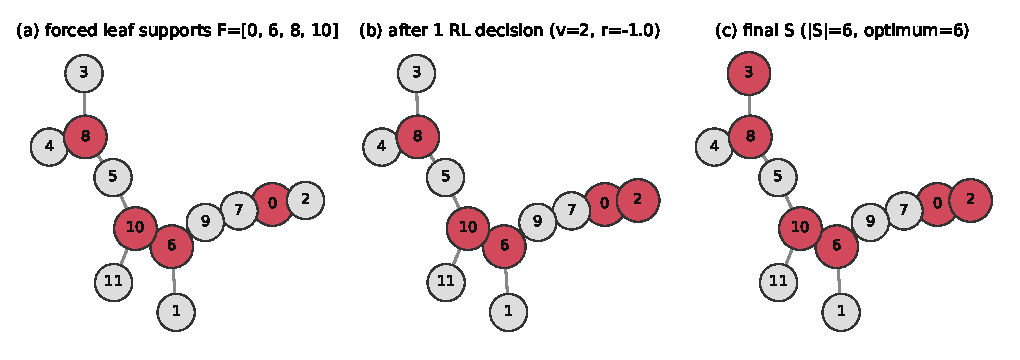
\includegraphics[width=0.98\textwidth]{figs/fig5_12_trace.pdf}
  \caption{اجرای گام‌به‌گام روی درخت $n=12$: (الف) نشاندن $F$؛ (ب) پس از یک تصمیم
  شبکه؛ (ج) مجموعه نهایی.}
  \label{fig:trace}
\end{figure}

\section{تهدیدهای اعتبار}
\label{sec:threats}

\begin{enumerate}
  \item \textbf{تعداد تکرار روی گراف‌های تصادفی:} برای \lr{ER} و \lr{BA} تنها
        \num{10} نمونه در هر اندازه تولید شده است (کمتر از آزمایش‌های فصل چهارم
        که \num{20} نمونه داشت). لتیس‌ها تک‌نمونه‌اند و نتیجه‌گیری قوی روی مثلثی
        مجاز نیست (تنها یک نمونه).
  \item \textbf{حل دقیق فقط تا $n\le120$:} بنابراین برای گراف‌های \lr{BA/ER}
        با $n=300$ و درخت‌ها با $n=200$، معیار $\gamma_t$ در دسترس نیست و مقایسه
        فقط با خط مبنای حریصانه انجام شده است.
  \item \textbf{تک‌seed بودن مدل‌های متراکم:} $size-v2$ و $paper-v2$ فقط با
        یک seed آموزش دیده‌اند؛ سه-seed فقط برای دو بازوی اسپارس انجام شده است.
        بنابراین ادعای «کیفیت» روی این دو \lr{checkpoint} به seed حساس است و در
        متن با همین قید نقل می‌شود.
  \item \textbf{معیار آستانه‌ای همگرایی:} عدد «$1.7$ برابر سریع‌تر» برای
        \lr{D3QN} بر پایه رسیدن به یک سطح آستانه تعریف شده و به انتخاب سطح فلات
        حساس است.
  \item \textbf{roll-out قطعی:} در ارزیابی، تصمیم‌گیری روی مقادیر $Q$ و بدون
        نمونه‌گیری انجام می‌شود؛ بنابراین نوسان تصادفی در نتایج آزمایش وجود ندارد
        و تنها منبع تصادفی، خودِ نمونه‌های گراف و کنترل \lr{random@k} است.
\end{enumerate}
